\section{Bayesian correlation paths}
The first 104 weekly returns (2003-08-15--2005-08-05) are reserved for initial-prior calibration and excluded from the Bayesian likelihood. Descriptive tables retain the full data sample. Parameters were estimated using 2005-08-12--2026-09-04; the model was saved at 2026-09-27T09:08:55.845Z (UTC). State smoothing uses observations through 2026-09-04. The posterior-mean parameter estimates stay fixed while the mean, volatility and correlation states are jointly smoothed over the modeled period. These bands show state uncertainty conditional on the saved posterior-mean parameters; they exclude parameter uncertainty. Historical state estimates can change when later observations are included.\par
{\footnotesize\raggedright Saved parameter file:\par\ttfamily /\allowbreak{}Users/\allowbreak{}jrubior/\allowbreak{}Documents/\allowbreak{}GitHub/\allowbreak{}DSC-\allowbreak{}AC-\allowbreak{}model/\allowbreak{}outputs/\allowbreak{}weekly\_\allowbreak{}research/\allowbreak{}parameters/\allowbreak{}dsc\_\allowbreak{}parameters\_\allowbreak{}20260927T090855845Z\_\allowbreak{}0286d4ba-\allowbreak{}f106-\allowbreak{}4588-\allowbreak{}bd10-\allowbreak{}c52848277526.mat\par}
The selected sampler run retained 828 draws pooled across 4 original chain(s), after discarding 20 warm-up iterations per chain. The dark line is the posterior median of the actual correlation $P_{ij,t}$ and the gray envelope contains the pointwise 16th and 84th percentiles. Vertical colors use the same continuous scale as Figure~1: blue for negative values, white near zero, and red for positive values, with intensity set by the posterior median. State-chain convergence has not been established, so the bands are preliminary. Parameter-estimation diagnostic status: not\_checked. State-smoothing diagnostic status: failed. Across 130,900 checked quantities, maximum rank-normalized split $\widehat R$: 2.715; minimum bulk/tail effective sample sizes: 4.853/11.03; maximum mean Monte Carlo error relative to sample standard deviation: 0.4712. Unequal retained counts: aligned diagnostics are exploratory because pooled summaries use all retained draws.
\begin{figure}[p]\centering
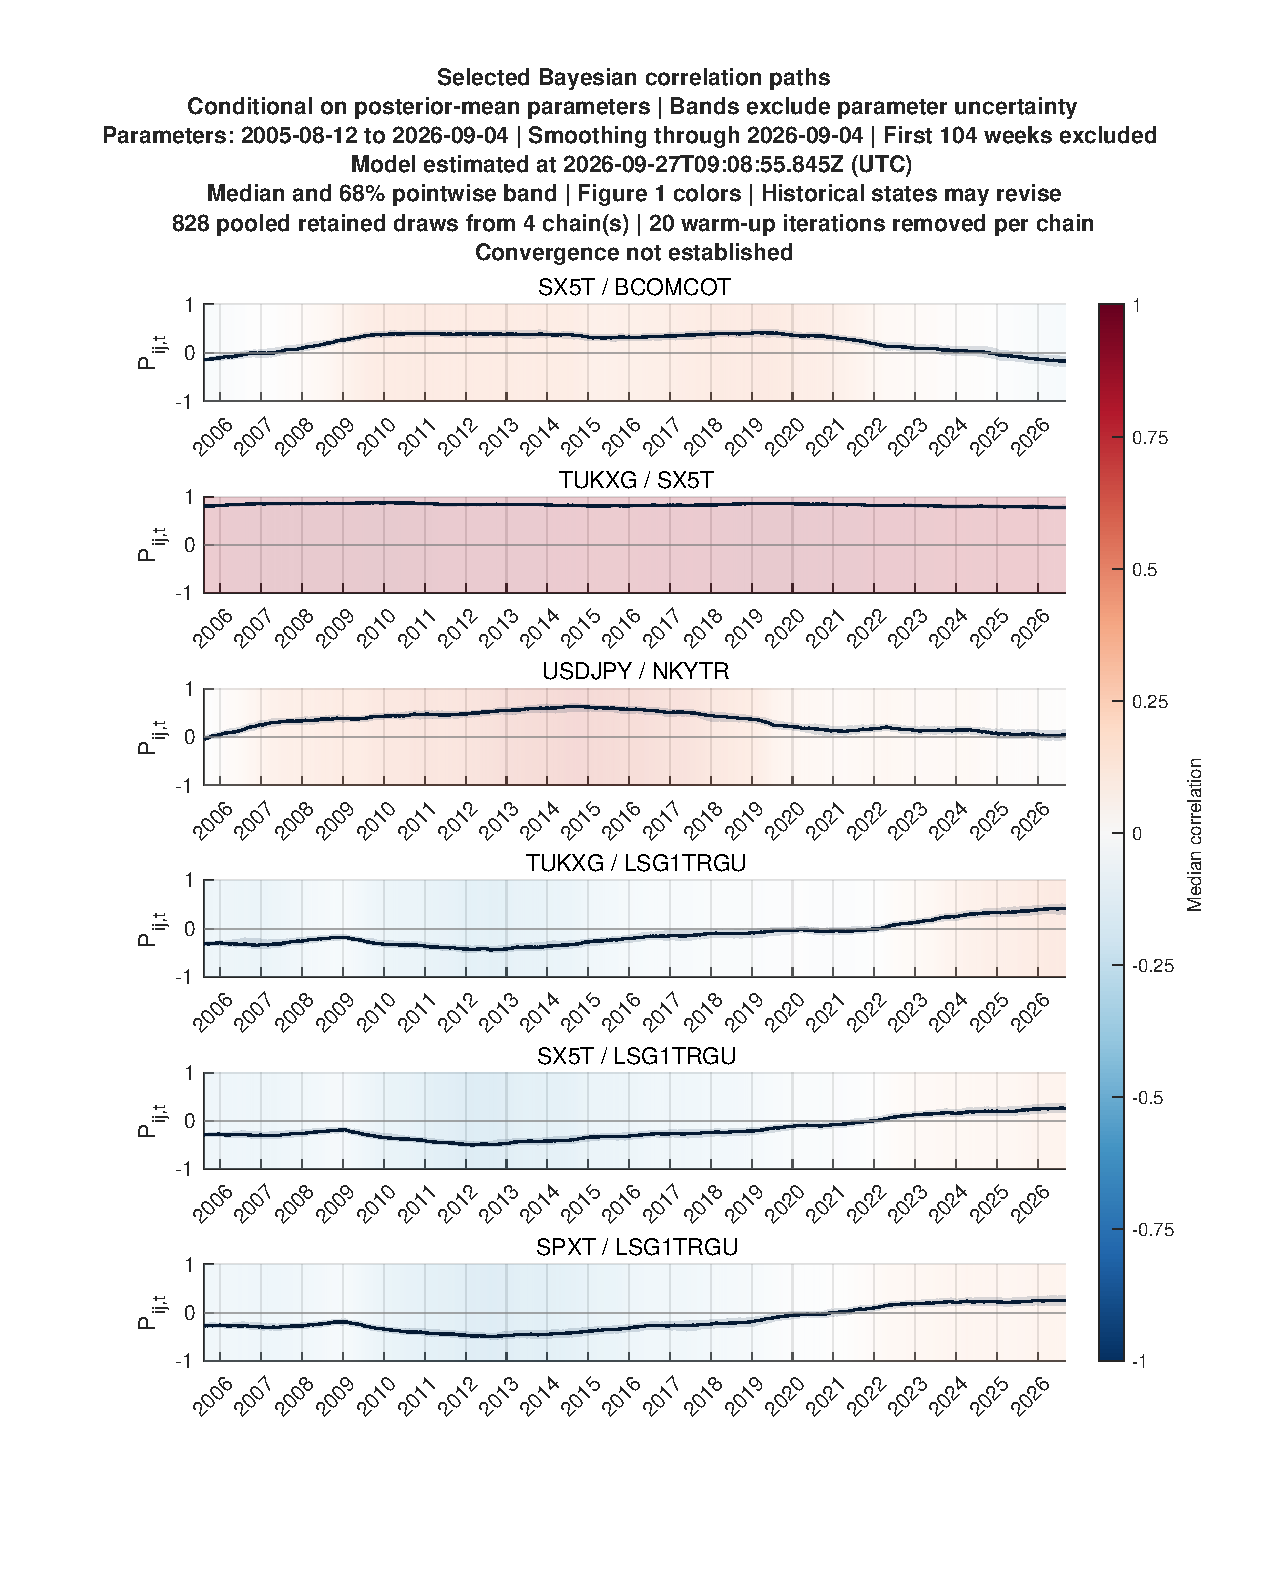
\includegraphics[width=\linewidth,height=.80\textheight,keepaspectratio]{generated/figures/bayesian_paths_selected.pdf}
\caption{Selected smoothed conditional innovation-correlation paths. The intervals are pointwise 68\% conditional posterior bands with posterior-mean parameters fixed; they exclude parameter uncertainty and are not simultaneous bands.}
\end{figure}
\clearpage
\textbf{Companion figure file.} The complete set of 91 Bayesian correlation paths is generated as \texttt{weekly\_correlation\_paths.pdf}. Each page uses the same vertical scale, color scale, and posterior summaries for every pair.\par
\clearpage
